Describe here work that is connected to your thesis. This should include
references to published work. There is no fixed rule, but I would expect a
student to have read around 50 published research papers and reference them in a
thesis.

\section{Evaluation metrics}

For multiclass classification problems, e.g.\ identifying a sample as a
particular bird species from a last of $n > 2$ species, a simple classification
accuracy is often used as an evaluation metric
(\cite{chakraborty2016bird},~\cite{ramashini2022robust}). This is calculated as
the percentage of correctly identified samples from a set of labelled samples
previously unseen by the model.

Acevedo et al~\cite{acevedo2009automated} used true positive ($TP$) and false
positive ($FP$) rates to evaluate their models used to classify bird and amphibian
calls. This evaluation method is sometimes preferred when analysing long
recordings which may include several different species to be classified. $TP$
gives an indication as to how well the model correctly identifies species
present in the recording. $FP$ indicates how often the model erroneously
identifies species absent in the recording. A high performing model will have
high values for $TP$ and low values for $FP$\@.

Potamitis et al~\cite{potamitis2014automatic} used an alternative form of
evaluation presented in terms of precision $(P)$ and recall $(R)$ which are
defined as
\begin{equation}
  P = \frac{\text{TP}}{\text{TP}+\text{FP}}, \hspace{1em}
  R = \frac{\text{TP}}{\text{TP}+\text{FN}}
\end{equation}
where $FN$ is the number of false negatives. Informally, $P$ and $R$ can be
thought of as
\begin{equation}
  P = \frac{\text{relevant retrieved instances}}{\text{all \textbf{retrieved} instances}}, \hspace{1em}
  R = \frac{\text{relevant retrieved instances}}{\text{all \textbf{relevant} instances}}
\end{equation}
It's well known that there is usually a trade-off between $P$ and $R$, so
usually the $F$-score is reported along with the $P$ and $R$ metrics. The
$F$-score is defined as
\begin{equation}
F = \frac{(1+\beta^2)PR}{\beta^2P + R}
\end{equation}
for some $\beta \in \mathbb{R}$.

For binary classification problems, i.e.\ classifying a sample as one of two
classes (bird species), the Area Under Curve (AUC) metric is sometimes
preferred~\cite{leng2014multi}. The AUC ranges from 0 to 1, with a higher value
indicating a better performing model. The AUC is sometimes desirable because it
is scale-invariant (it measures how well predictions are ranked, rather than
their absolute values) and classification-threshold-invariant (it measures the
quality of the model's predictions regardless of what classification threshold
is chosen.)

\section{Feature extraction}

As mentioned in Chapter~\ref{cp:intro}, birds use vocalizations as a way to
communicate with others. Birds have evolved over many thousands of years to
make this form of communication very efficient in that it can travel long
distances and cut through local ambient noise frequencies so that it can be
received by other birds clearly. Some birds have even adapted their
vocalizations so that they can be heard in local environments that have rapidly
changed over the past decades, such as urban areas with increasing anthropogenic
noise~\cite{luther2010urban}.

Bird vocalizations can be broadly divided into two main categories, calls and
songs. Calls are typically short vocalizations that carry some specific
function, such as warning others to the presence of a predator or calling others
to flight~\cite{MARLER2004132}. Songs are usually longer and more acoustically
complex and occur more spontaneously. Songs are typically employed as breeding
calls or territorial defence. While all birds produce calls, in many species of
birds only the males utilise songs and often only during breeding season. The
song and call of a Eurasian Wren can be seen and contrasted in
figure~\ref{fig:wren_call_song_spectrogram}.

Doupe et al~\cite{birdsongspeech} showed that there were striking similarities
between birdsong and human language. Similar to human language, birdsong can be
thought of as comprised of hierarchical levels of phrases, syllables, and
elements~\cite{catchpole2003bird}. <Figure here>. Raw recordings of birdsong
often contain periods of silence that occur between phrases which are unlikely
to provide useful information in order to train a machine learning model.
Fagerlund~\cite{fagerlund2007bird} showed that a good level of accuracy can be
achieved by training models on features extracted from segmented syllables which
were used as training samples. An algorithm for robust syllable segmentation was
proposed in~\cite{fagerlund2004automatic} and is used in this thesis. The
algorithm is described in more detail in Section.

\begin{figure}[ht]
  \centering
  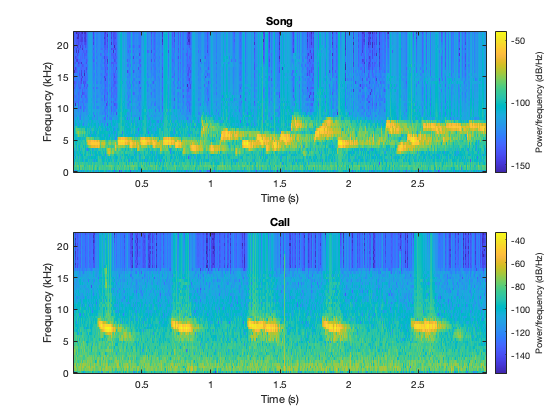
\includegraphics[width=\textwidth]{figures/wren_call_song_spectrogram.png}
  \caption{Spectrograms of the call and song of the Eurasian Wren
    (\textit{Troglodytes troglodytes}). As can be seen, the song is much more complex in terms of pitch and acoustic structure compared to the
  call}\label{fig:wren_call_song_spectrogram}
\end{figure}

Once the syllables have been segmented, there exists an abundance of options to
turn the raw syllable input signal into features that might be used as training
samples. In the following sections some of the more popular feature
representations are described, along with some novel methods that have yet to be
tried on birdsong. Note that the following list is certainly not exhaustive and
emphasis has been placed on feature representations that are relevant to this
thesis.

\subsection{Features inspired by the human auditory system}

Research has shown that birdsong and human language share many similarities in
terms of the neural mechanisms employed to form the language/song, the impact of
social contact in learning the language/song, and so on~\cite{birdsongspeech}.
Give that the human auditory system has evolved other thousands of years to best
process human speech, it seems reasonable to suggest that using features based
on the human auditory system may be effective when it comes to birdsong.

At a high level, the human auditory system works by translating changes in air
pressure originating from a source and reaching the outer ear of a listener
into vibrations that travel along an internal organ known as a cochlear. The
vibrations trigger electric signals that move along auditory nerves to the
brain, where they are interpreted as sounds. The physiology of the cochlear
means that certain parts of the organ are more sensitive to certain frequencies
of vibrations, so different frequencies will lead to different electrical
signals moving to the brain. This allows the brain to learn to differentiate
between frequencies.

\subsubsection{Mel frequency cepstrum coefficients}

The makeup of the human auditory system means that humans have a greater ability
to differentiate pitch at lower frequencies then they do at higher frequencies.
In other words, humans perceive pitch non-linearly. This has led to the
development of a logarithmic scale, known as the mel scale, such that equal
distances on the scale have the same \textit{perceptual} distance.

The mel frequency cepstrum coefficients (MFCC) are part of a family of cepstrum
coefficients that capture information about the rate of change in different
spectrum bands. MFCC differs from other cepstrum coefficients in that it uses the
mel scale to transform the spectrum of an input signal, thus utilising the human
auditory system in the calculation of its coefficients.

The $i$-th mel cepstral coefficient is computed as~\cite{davis1980comparison}
\begin{equation}
\text{MFCC}_i = \sum_{k=1}^{K} X_k \cos \left(
  \frac{i(k-0.5)\pi}{K}
\right)
\end{equation}
where $X_k$ is the logarithmic energy of the $k$-th mel-spectrum band, and $K$
is the total number of the mel-spectrum bands. Usually 8--13 MFCC coefficients
are used as the feature vector representing one time frame of the signal. The
0$^{th}$ coefficient is often excluded as it represents the average log energy
of the signal and is unlikely to carry any relevant information to help with
classification.

MFCCs are often presented with their delta ($\Delta$) and double-delta
($\Delta\Delta$) values that capture the local temporal dynamics and temporal
changes of the delta values respectively.

MFCCs are used as feature representations since they are simple to compute and
have been shown to have good performance in a wide range of audio classification
tasks, such as speaker identification~\cite{muda2010voice} and emotion
recognition~\cite{likitha2017speech}. MFCCs have also been shown to lead to good
classification accuracy for birdsong identification problems
(\cite{fagerlund2007bird} and~\cite{ramashini2022robust}).

<include graph of filterbank>

\subsubsection{Gammatone cepstrum coefficients}

Gammatone cepstrum coefficients (GTCCs) are similar to MFCCs except their
calculation  uses gammatone filterbanks instead of mel scale filterbanks.
Gammatone filterbanks are designed to simulate the motion of the membrane inside
the cochlear, known as the basilar membrane, when it is exposed to vibrations
transmitted by the outer and middle ear~\cite{patterson1992complex}.

A gammatone filter with a centre frequency $f_c$ is defined as
\begin{equation}
  g(t) = at^{n-1}e^{-2\pi b t} \cos(2\pi f_c + \psi)
\end{equation}
where $t$ is the time in seconds, $\psi$ is the phase in radians (usually set to
0), $a \in \mathbb{R}$ controls the gain, $n$ is the filter's order and $b$ is
the filter's bandwidth in Hz. To simulate the human auditory system, the centre
frequencies are uniformly spaced on the equivalent rectangular band-width (ERB)
scale.

Similar to MFCCs, GTCCs are typically used with their $\Delta$ and $\Delta\Delta$
values and have also been shown to have a good performance in
non-speech audio classification problems~\cite{valero2012gammatone}.

<include graph of filterbank>

\subsubsection{Multi resolution cochleagram}

Chen et al~\cite{chen2014feature} proposed a novel feature known as a
multi-resolution cochleagram (MRCG) that is formed by combining four
cochleagrams at different resolutions, designed to capture both local and
contextual information.

A cochleagram is formed by passing an input signal through a gammatone
filterbank, similar to the first steps of the formation of the GTCCs\@. Each
response signal from the gammatone filterbank is then divided into frames of a
certain length with a certain overlap or frame shift. The cochleagram is then
generated by calculating the power of each frame at each channel.

<example cochleagram>

A MRCG is formed by first taking one cochleagram with a frame length of 20ms and
frame shift of 10ms, using a gammatone filterbank with 64 output channels. A log
operation is applied to each time-frequency (T-F) unit of the output
cochleagram, denoted CG1. CG2 is calculated in the same way, but with a frame
length of 200ms and the same frame shift. CG3 is calculated by averaging CG1
across a square window of 11 frequency channels and 11 time frames centred at
the given T-F unit. Zero padding is used here. CG4 is calculated in the same way
as CG3, but with a $23 \times 23$ square window. CG1--4 are then stacked
vertically to obtain the full MRCG feature, which will be a $256 \times p$
matrix, where $p$ is the number of time frames.

<example mrcg>

The MRCG feature has been shown to outperform both MFCC and GTCC at
separating human speech at various SNR levels with different types of
background noise~\cite{chen2014feature}. Abdullah et
al~\cite{binti2020comparison} showed that the MRCG outperforms the Auditory
Image Model (AIM) when classifying noise. Wang et al~\cite{wang2016joint} showed
that improved speech enhancement for hearing impaired listeners was achieved
when the MRCG feature was added to the feature set.

One potential drawback when comparing the MRCG with MFCC and GTCC is the higher
dimensionality of the MRCG feature. When including the $\Delta$ and
$\Delta\Delta$ features, as is standard practice
(\cite{binti2020comparison},~\cite{wang2016joint}), the MRCG feature vector for
a single time frame has a dimensionality of 768. For MFCC or GTCC the equivalent
dimensionality is 24--39, depending on the number of the coefficients used.

\subsection{Feature stacking}

It has been shown that combining features to be used as training inputs can lead
to improved classification accuracy. Ramashini et al~\cite{ramashini2022robust}
showed that a combination of GTCC and MFCC yielded higher birdsong classification
accuracy than MFCC alone. However, the combination did not improve on the
accuracy of GTCC alone. Yan et al~\cite{yan2021birdsong} demonstrated that a
combination of MFCC with two other feature types (Log-mel spectrogram and
Chroma) yielded higher birdsong classification accuracy than combinations of two
of the features alone. Fagerlund~\cite{fagerlund2007bird} showed that combining
MFCC with spectral and temporal features, such as frequency range and zero
crossing rate, can lead to higher birdsong classification accuracies.

A consequence of feature stacking is that feature vectors will have increased
size. This can lead to problems such as longer training times and overfitting,
especially when used in conjunction with deep learning architectures. As a
result, dimensionality reduction techniques, such as Principal Component
Analysis (PCA) or Linear Discriminant Analysis (LDA)~\cite{ramashini2019bird},
are often used to lower the dimensionality of the feature vectors while still
capturing enough information to be able to train a model effectively.

\section{Classification}

Once a suitable feature representation has been selected and performed, the
remaining task is to pick an appropriate model and train the model using the set
of training samples generated from the feature extraction.

There exist many different options in terms of models, and no one model is
superior to the others. Each problem must be considered and a model which fits
the problem at hand must be selected, or indeed a selection of suitable models
tested and the evaluated for performance.

In the literature, birdsong classification has been tackled with a wide variety
with models. Ramashini et al~\cite{ramashini2019bird} used the simple Nearest
Centroid (NC) classifier to assign birdsong samples to classes. It was compared
to a K Nearest Neighbours (KNN) classifier and shown to have superior accuracy.
Lasseck~\cite{lasseck2015improved} used decision trees with bagging to identify
birds. Trifa et al.~\cite{trifa2008automated} used Hidden Markov Models (HMM) to
identify species of birds based on their vocalizations. They considered each
sample as a discrete-time dynamical system, where an unobserved state generates
observed features, such as pitch and MFCC\@. A different HMM can be learned for
each class and a new sample can be assigned to a class by calculating which HMM
gives the highest likelihood of the observed features. Kwan et
al.~\cite{kwan2006automated} used a Gaussian Mixture Model (GMM) to classify
birds. In their experiments, a Gaussian was learned for each class of bird. A
new sample was then classified according to whichever class best describes the
new sample.

The following sections describe some models that are relevant to this thesis in
more detail

\subsection{SVMs}

SVMs are widely used in machine learning applications as a classification tool.
They are well-established due to their high accuracy
results~\cite{fagerlund2007bird} and relative simplicity to implement. Most
implementations of SVMs also require little or no tuning of hyperparameters.

At its core, a SVM is a binary classifier that separates two classes by finding
a hyperplane that maximizes the margin from the nearest vectors in the feature
space from both classes. Classifications are then made by computing in which
side of the hyperplane a test feature vector lies.

\subsubsection{Binary classification}

Let $\mathbf{x}_i \in \mathbb{R}^m$ be a feature vector of dimensionality $m$.
Let $y_i \in \left\{ +1, -1 \right\}$ be its class label. For linearly separable
data, the separating hyperplane satisfies
\begin{equation}\label{eq:svm_hyperplane}
y_i\left( \left< \mathbf{w} \cdot \mathbf{x}_i \right> + b \right) \ge 1, \hspace{1em}
i = 1,\ldots,n
\end{equation}
where $\mathbf{w} \in \mathbb{R}^m$ is a vector of weights and $b \in
\mathbb{R}$ is a bias term. The margin between the hyperplane and the nearest
feature vectors from each class is given by
\begin{align}
  \text{d}(\mathbf{w},b) &=
  \min_{\mathbf{x}_i,y_i=1}
  \frac{|\left< \mathbf{w} \cdot \mathbf{x}_i \right> + b|}{\|\mathbf{w}\|} +
  \min_{\mathbf{x}_j,y_i=-1}
  \frac{|\left< \mathbf{w} \cdot \mathbf{x}_j \right> + b|}{\|\mathbf{w}\|} \\[0.5em]
                         &= \frac{2}{\|\mathbf{w}\|}. \label{eq:svm_margin}
\end{align}

The optimal hyperplane can now be found by maximizing (\ref{eq:svm_margin})
subject to (\ref{eq:svm_hyperplane}). This can be solved using Lagrange
multipliers.

Often with real world data, classes are not linearly separable. This can
remedied by projecting the data using a nonlinear mapping into a new feature
space where the data are linearly separable. Equation (\ref{eq:svm_hyperplane})
can then be re-written as
\begin{equation}\label{eq:svm_nonlinear_mapping}
y_i\left( \left< \mathbf{w} \cdot \boldsymbol{\Phi}(\mathbf{x}_i) \right> + b \right) \ge 1, \hspace{1em}
i = 1,\ldots,n
\end{equation}
where $\boldsymbol{\Phi}$ is the nonlinear mapping. Instead of explicitly
finding $\boldsymbol{\Phi}$, (\ref{eq:svm_nonlinear_mapping}) can be re-written
in dual form
\begin{equation}
y_i\left(
  \sum_{j=1}^{l} \alpha_j y_j \left<
  \boldsymbol{\Phi}(\mathbf{x}_j) \cdot \boldsymbol{\Phi}(\mathbf{x}_i)
  \right>
\right) + b \ge 1, \hspace{1em} i=1,\ldots,n
\end{equation}
and replacing the inner product with a kernel function
$K(\mathbf{x}_j,\mathbf{x}_i) = \left< \boldsymbol{\Phi}(\mathbf{x}_j) \cdot
\boldsymbol{\Phi}(\mathbf{x}_i) \right>$.

In practice, a hyperplane that separates the classes perfectly may suffer from
poor generalization ability. To improve this, nonnegative slack variables
$\xi_i$ are introduced to (\ref{eq:svm_nonlinear_mapping}) to allow for some
missclassification of training samples in order to improve generalization
ability. The slack variables are introduced like so
\begin{equation}\label{eq:svm_nonlinear_mapping_slack}
y_i\left( \left< \mathbf{w} \cdot \boldsymbol{\Phi}(\mathbf{x}_i) \right> + b
\right) \ge 1 - \xi_i, \hspace{1em}
i = 1,\ldots,n
\end{equation}
The amount of regularization is controlled by the constant $C$ such that the
maximization problem (\ref{eq:svm_margin}) becomes
\begin{equation}
\frac{2}{\|\mathbf{w}\|} - C \sum_{i=1}^{n} \xi_i
\end{equation}

Therefore for large values of $C$ the classifier will behave like a hard-margin
SVM and attempt to perfectly classify all training samples.

The last remaining question is around what determines a valid kernel function. A
function in the input space is a kernel function if its kernel matrix
$\mathbf{K} = \left[ K(\mathbf{x}_j,\mathbf{x}_i) \right]^{n}_{i,j=1}$ is
positive semidefinite. Typical kernel functions include
\begin{itemize}

  \item linear: $K(\mathbf{x}_j,\mathbf{x}_i) = \left< \mathbf{x}_j, \mathbf{x}_i \right>$

  \item polynomial: $\left(\left< \mathbf{x}_j, \mathbf{x}_i \right> + c\right)^p$
    for some $c \in \mathbb{R}$

  \item Gaussian or RBF\@: $\exp \left( -\gamma \|\mathbf{x}_j-\mathbf{x}_i\|^2 \right)$
    for some $\gamma \in \mathbb{R}, \gamma > 0$.

\end{itemize}

\subsection{Neural Networks}

Although neural networks have existed in some form since the 1950s with
inception of the perceptron algorithm~\cite{rosenblatt1958perceptron}, they have
experienced a huge surge in popularity over the past decade or so. This has
largely been due to remarkable progress being made thanks to deep neural
networks in fields such as image classification~\cite{krizhevsky2012imagenet}
and language models~\cite{mikolov2010recurrent}.

Another reason for deep learning's increasing popularity in recent years is due
to the availability of more performant hardware and software. The `deep' aspect
to deep learning refers to the fact that the software architecture depends on
large amounts of parameters and needs massive amounts of training data in order
to learn. In order to run training routines in a reasonable time and store large
amounts of data in memory, access to powerful hardware and/or machine
parallelism tools can be an essential part of the process.

The progress of audio problems related has also been accelerated due to deep
neural networks. Hinton et al.~\cite{hinton2012deep} showed improved performance
in speech recognition tasks using feed-forward neural networks when compared to
more classical approaches like HMMs and GMMs. Speech
enhancement~\cite{afouras2018conversation} and speech
separation~\cite{ephrat2018looking} problems leveraging deep learning paradigms
have also been shown to outperform more classical statistical models. The
world of birdsong classification has also benefited from deep learning, but
perhaps to a lesser extent than other audio related problems so far.

\subsubsection{Feedforward Neural Network}

\subsubsection{Convolutional Neural Network}

\subsubsection{Recurrent Neural Network}
